\section{Architecture}
\label{sec:Architecture}
\subsection{Activity(android)}

\subsection{Architecture model}
The WOMBAT application is depended on the Launcher project and Oasis project, but we choose to design WOMBAT as an independent application with features from Launcher and Oasis.
We choose to design WOMBAT as an independent application, that way we never have to wait for the Launcher or Oasis to release features regarding WOMBAT. You can see a dependency diagram of WOMBAT architecture. The WOMBAT architecture is a five layer architecture which enhances how you can perform testing and do collaborative work. The five layers consists of: 

\begin{figure}[H]
	\centering
		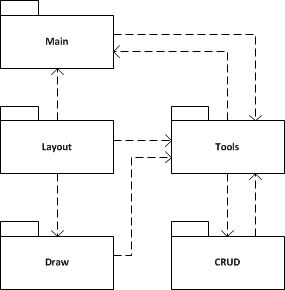
\includegraphics[scale=0.6]{Images/Implementation/WombatDependency.png}
	\caption{Dependecy diagram of WOMBAT architecture}
	\label{fig:WombatDependency}
\end{figure}


\begin{itemize}
	\item[Main] \hfill \\	This layer is the main activity of WOMBAT which means that it initiate the whole WOMBAT application. The main layer is depended on the Tools layer since it contains all the initiating tools. 
	\item [Layout] \hfill \\	This layer cosists of the two fragments; Profile/SubProfile fragment and customize fragment, and the custom arrayadapters which WOMBAT uses. The layout layers is depended on the Tools since it contains all the objects and methods that is required for the layout to work properly. The layout layer is also depended on the main layer, without the main layer the layout layer would never be initiated. Final but no least the layout layer is depended on the draw layer, the draw layer delivers the methods that generates the views for the timers and pictograms.
	\item [Draw] \hfill \\	This layer contains the methods that generate the views of timers and pictograms. Draw layer is depended on the tools layer since the tools layers contain all the different types of objects that the draw layer uses. The draw layer is also depended on the layout layer, the layout layer initiate the draw layer.
	\item [Tools] \hfill \\	This layer cosists of all the types of objects and methods that WOMBAT uses. The tools layer is depended on the main layer to initiate the proper objects, you can read more about this in subsection: \ref{subsec:TimerLib}. The tools layer is also depended on the CRUD layer which contains the connection to the Oasis library.
	\item [CRUD] \hfill \\	This layer is responsible for saving and loading from the OasisLocalDatabase, it is depended on the tools layer because it uses the objects and method that the tool layer provides.
\end{itemize}

\subsubsection{Library}

Our original idea was the split the layers into two projects, that way it would be able to conduct tests outside the main layer. The first project would be an Android project with a main activity, WOMBAT. The second project would be an Android library which should contain all the backend functionality, TimerLib. This is how it the two projects would look like:

\begin{description}
  \item[WOMBAT] \hfill \\\begin{itemize}  \item Main layer  \item Layout layer
\end{itemize}
  \item[TimerLib] \hfill \\\begin{itemize}  \item Tools layer  \item Draw layer  \item CRUD layer
\end{itemize}
\end{description}

We later decided to redesign, and make three projects instead of two projects. We choose the redesign because that we are three developers in our project whom all want to conduct independent testing. The first project, WOMBAT, would stay as it original was. The Second project would be split into two projects, TimerLib and DrawLib. TimerLib would contain the tools layer and the CRUD layer. The DrawLib would contain the draw layer.

\begin{description}
  \item[WOMBAT] \hfill \\\begin{itemize}  \item Main layer  \item Layout layer\end{itemize}
  \item[TimerLib] \hfill \\\begin{itemize}  \item Tools layer  \item CRUD layer
\end{itemize}
  \item[DrawLib] \hfill \\\begin{itemize}  \item Draw layer\end{itemize}
\end{description}

The dependency diagram of the WOMBAT projects can be see on figure: \ref{fig:LibraryDependency}.

\begin{figure}[H]
	\centering
		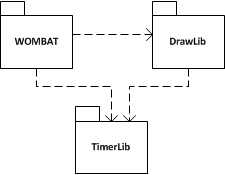
\includegraphics[scale=0.6]{Images/Implementation/LibraryDependency.png}
	\caption{Dependecy diagram of WOMBAT projects}
	\label{fig:LibraryDependency}
\end{figure}

\subsubsection{Wombat lifecycle}
You can see a detailed flowchart over the WOMBAT lifecycle on figure:\ref{fig:wombatLifeCycle}. The flowchart descrips whatever that can occur while the WOMBAT application is running. The flowchart can help debug and understand the application if somebody chooses to develop futher on WOMBAT.

\begin{figure}[H]
	\centering
		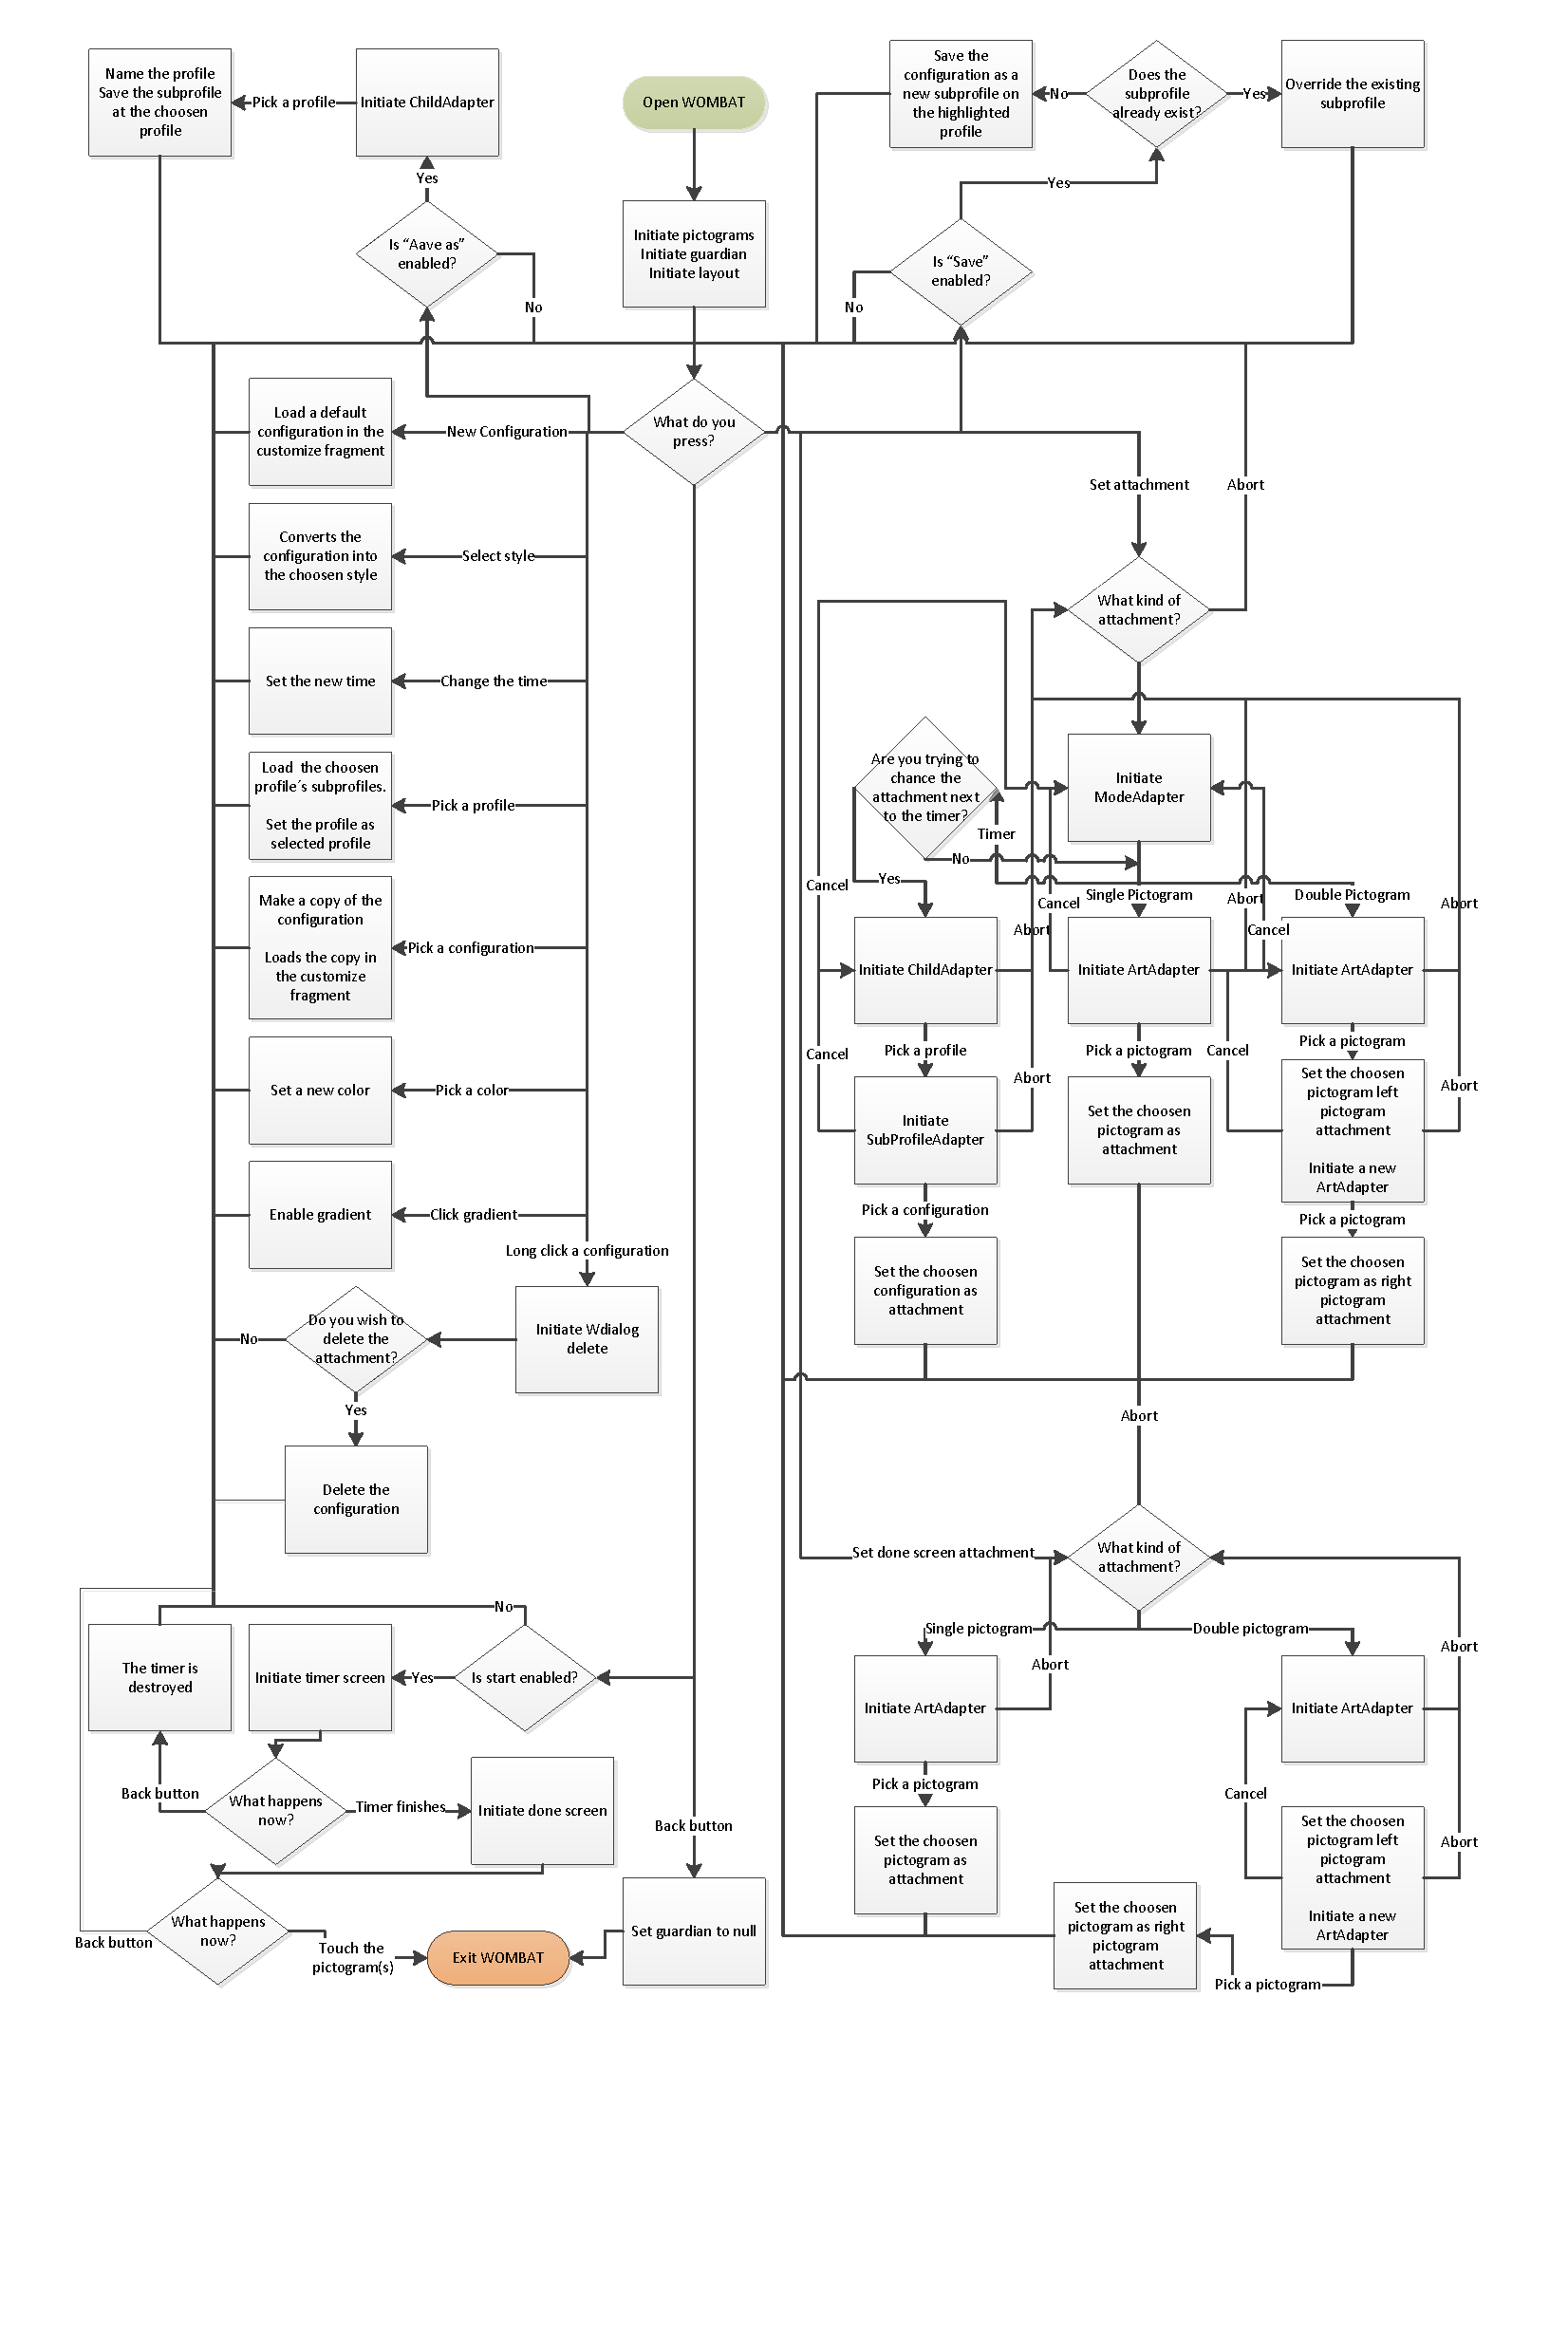
\includegraphics[scale=0.6]{Images/Implementation/wombatLifeCycle.pdf}
	\caption{Flowchart of WOMBAT lifecycle}
	\label{fig:wombatLifeCycle}
\end{figure}